\documentclass[10pt,twocolumn]{article}

\usepackage[ruled,vlined]{algorithm2e}
\usepackage{tikz}
\usepackage{amsmath}
\usepackage{amssymb}
\usepackage{color}
\usepackage[thmmarks,standard,thref]{ntheorem}
\usepackage[headheight=15pt,lmargin=1cm,rmargin=2cm,tmargin=2cm,bmargin=3cm]{geometry}
\usepackage{semantic}



\usetikzlibrary{shapes,trees,arrows,snakes,backgrounds}
\tikzstyle{root}=[rectangle,draw=black!50,thick,minimum size=6mm]
\tikzstyle{var}=[circle,draw=black!50,thick,minimum size=6mm]
\tikzstyle{n}=[->,dashed,thick]
\tikzstyle{p}=[->,thick]

\bibliographystyle{abbrv}



\newcommand{\C}[1]{\mathcal{#1}}

\newcommand{\TODO}[1]{\textcolor[rgb]{1.00,0.00,0.00}{#1} }

%\begin{document}
\title{Maintaining GAC via UP on CNF encodings from BDDs and sDNNFs}
\author{Jean Christoph Jung \and Valentin Mayer-Eichberger}



\begin{document}
\date{\today}

\maketitle 

%\tableofcontents  


\section{Definitions}

\begin{definition}
We are working with the following structures:

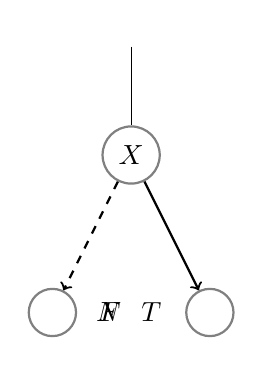
\begin{tikzpicture}
\centering
    \node[var] (1) at (0,2) {$X$};
    \node[var] (2) at (-1,0) {$ $};
    \node[var] (3) at (1,0) {$ $};
    \node (0) at (0,3.5) {};
    \draw (0) to (1) node[pos=0.8,left] {$N$}; 
    \draw[n] (1) to (2) node[pos=0.8,left] {$F$}; 
    \draw[p] (1) to (3) node[pos=0.8,right] {$T$};
   \end{tikzpicture}   

\begin{itemize}
\item Syntax: 
   \begin{itemize}
    \item BDD node $N$ is tuple: $\langle N,X,T,F \rangle$ 
    \item Set of nodes $\mathcal{N}$
    \item Set of variables $\mathcal{V}$ with total order $\prec$ and successor operations (s(X) = X+1) 
    \end{itemize}
\item Rules: 
    \begin{description} 
        \item[SINK] Let $M = max(\mathcal{V})+1$, there are to distinct unique sinks $0,1 \in \mathcal{N}$ with:
            \begin{align*}
            & \langle 0,M,1,0 \rangle \\
            & \langle 1,M,1,0 \rangle \\
            \end{align*}
        \item[EXIST] $\forall N \in \mathcal{N}$
            \[
            \exists T,F \in \mathcal{N}  \exists X \in \mathcal{V}. \langle N,X,T,F \rangle \\  
            \]
        \item[UNIQUE] $\forall T,F \in \mathcal{N} \;  \forall X \in \mathcal{V} \exists N_1,N_2 \in \mathcal{N}$
            \[
            \langle N_1,X,T,F \rangle \wedge \langle N_2,X,T,F \rangle \text{ then } N_1 = N_2
            \]
        \item[REDUNDANT] $\forall H \in \mathcal{N} \;  \forall X \in \mathcal{V}$
            \[
             \neg \exists N \in \mathcal{N} \text{ s.t.} \langle N,X,H,H \rangle 
            \]
        \item[ORDER] $\forall N,T,F \in \mathcal{N} \;  \forall X,Y_1,Y_2 \in \mathcal{V} $
            \begin{align*}
            (\langle N,X,T,F \rangle \wedge \langle T,Y_T,\ast,\ast \rangle \wedge \langle F,Y_F,\ast,\ast \rangle)\\
             \rightarrow (X \prec Y_T \wedge X \prec Y_F)
            \end{align*}       
%        \item[QUASI] $\forall N,T,F \in \mathcal{N} \;  \forall X,Y_1,Y_2 \in \mathcal{V} \;\;$
%             \begin{align*}
%             (\langle N,X,T,F \rangle \wedge \langle T,Y_T,\ast,\ast \rangle \wedge \langle F,Y_F,\ast,\ast \rangle) \rightarrow \\
%             (Y_T= X+1 \wedge Y_F = X+1)
%             \end{align*}
    \end{description}
\item Semantics: 
    \begin{description} 
        \item[FORMULA]
            \[
            N \rightarrow \left((X\rightarrow T)\wedge(\neg X\rightarrow F)\right)
            \]
    \end{description}
\end{itemize} 
\end{definition}

\begin{definition}
The tuple  $(\mathcal{V},\mathcal{N},R)$ is 
    \begin{description} 
        \item[BDD] if it obeys SINK and EXIST
        \item[ROBDD] if it is a BDD and obeys UNIQUE,REDUNDANT and ORDER
%        \item[QOBDD] if it is a BDD and obeys UNIQUE, and QUASI
%        \item[UPBDD] puhhh, this is hard
    \end{description}
\end{definition}


\begin{definition}
$[N_1,...,N_n]$ is a path iff $\forall N_i$ it holds $N_i \not = 0$ and $( 
(\neg X \wedge \langle N_i,X,\ast ,N_{i+1}\rangle) \vee (X \wedge \langle 
N_i,X,N_{i+1,\ast }\rangle )$
\end{definition}

NOTE IN THIS DEFINITION X IS FREE, if X has domain {0,1} we could use both 
descendants 

\begin{definition} $ $

\begin{itemize}
\item $N$ is reachable $P(N)$, iff there exists a path $[R,...,N]$
\item $N$ is consistent $C(N)$, iff there exists a path $[N,...,1]$
\end{itemize}
\end{definition}



\begin{definition}
BDD encoding is GAC wrt scope $(X_1,X_2...X_n)$ and their current domains IFF  
$\exists N_1,N_2,\ldots N_l \in \mathcal{N}$ such that $\forall X_1,X_2,\ldots 
X_n$ it holds $\bigwedge_{i=1}^l (C(N_i) \wedge P(N_i))$. 
\end{definition}


\section{BDD GAC Encoding}

\begin{definition}
Let $(\mathcal{V},\mathcal{N})$ be a ROBDD (possible shared). The set 
$\mathcal{N}$ contains the additional variables to describe a path 
$N_1,N_2,\ldots N_n$ through the BDD.  To construct a path we have several 
options to prepare it for the SAT solver, with different strength: 
\begin{description}
   \item[ROOT] Root is reachable, the 1 sink is true and the 0 sink is false:
    \begin{align*}
    R \wedge 1 \wedge \neg 0
    \end{align*}
  \item[BDD1] $N$ is reachable and  $X = 1$ ($X = 0$) then $T$ ($F$) is reachable
    \begin{align*}
    (N \wedge X) &\rightarrow T\\
    (N \wedge \neg X) &\rightarrow F\\
    \end{align*}
  \item[BDD2] 1) $N$ is reachable then one of the descendants is reachable. 2) If both 
descendants are not reachable, then $N$ is not reachable 
    \begin{align*}
    &N \rightarrow ( F \vee T)\\
    &(\neg F \wedge \neg T) \rightarrow \neg N\\
    \end{align*}
  \item[BDD3] 
    \begin{align*}
    (N \wedge T) &\rightarrow X\\
    (N \wedge F) &\rightarrow \neg X\\
    \end{align*}
  \item[PARENT] Let $P_1,P_2 \ldots P_k$ be all parents of node $N$. If non of parents is 
        reachable then N not reachable. Let $P_1,P_2 \ldots P_k \text{ with 
        } (\langle P_i,\ast,N,\ast \rangle \vee \langle P_i,\ast,\ast,N 
        \rangle)$ then 
    \[
    \bigwedge_{i=1}^k \neg P_i  \rightarrow \neg N
    \]
  \item[TOPDOWN] Let $ N_1,N_2 \ldots N_k \text{ with } \langle 
N_i,X,T_i,F_i\rangle$ and let $ Q_1,Q_2 \ldots Q_l$ s.t. $\exists Y,Z\in 
\mathcal{V}$ with  $Y \prec X\prec Z$ s.t.  $\langle 
Q_i,Z,\ast,\ast\rangle$ and $\exists P \in \mathcal{N}$ s.t. $\langle 
P,Y,Q_i,\ast \rangle$ or $\langle P,Y,\ast,Q_i \rangle$ then 
    \begin{align*}
\bigwedge_{i=1}^l \neg Q_i \rightarrow  \left(  \left( \bigwedge_{i=1}^k \neg F_i \rightarrow X  \right) \wedge \left(\bigwedge_{i=1}^k \neg T_i   \rightarrow \neg X  \right) \right)\\
    \end{align*}
\item[MAX] Max one is reachable in each level: Let $N_1,N_2 \ldots N_k \text{ with } \langle N_i,X,\ast,\ast\rangle$
    \[
    \bigwedge_{i \prec j} \neg N_i \vee \neg N_j
    \] 
  \end{description}  
  
\end{definition}

\section{LOCAL KNOWLEDGE rules}
\TODO{I guess we can change this section to work only with sDNNF, then ROBDD 
are a special case of it. so the rules have to be rewritten (possible simpler). 
(rule for local knowledge, rule for OR node, rule for AND node, rule for leaf)
} 

This is a more general approach (could work for sDNNF as well). We model
intersection and union with additional local knowledge variables. Node 
variables mean again \emph{being on the final path}.  

\begin{definition}
We define the occurring literals of a sDNNF subtree with root $N$ as follows 
\[
lit(N) = 
\begin{cases}
\{ L \}& \text{if $N$ is leaf and $L$ is its literal} \\
\bigcup_i lit(F_i) & \text{$F_1\ldots F_n$ children of $N$} \\
\end{cases}
\]
\end{definition}
    
Now for each node $N$ we introduce variables $N_Y$ for each $Y\in lit(N)$. They 
correspond to: $N_Y$ means that literal $Y$ is known in node $N$.  
    
  \begin{description}  
  \item[GLOBAL] Local knowledge at the root is global knowledge. 
    \begin{align*}
%    \forall Y \in lit(N)/\{X\} &\;\;\; Y \rightarrow N_Y \\
    \forall Y \in lit(R) &\;\;\; R_Y \rightarrow  Y\\
    \end{align*}  
  \item[INTERSECTION] Let $N$ be an OR node. Implications are propagated up, if they are known in 
all descendants $F_1 \ldots F_n$. $\forall Y \in lit(N)$ 
    \[
    \left(\bigwedge_{i=1}^n F_{i,Y}\right) \rightarrow N_Y
    \]  
  \item[UNION] Let $N$ be an AND node. Implications are propagated up, if they are known in one of the descendants $F_1 \ldots F_n$. $\forall Y \in lit(N)$ 
    \[
    \left(\bigvee_{i=1}^n F_{i,Y}\right) \rightarrow N_Y
    \]  
%  \item[INTRO] Local knowledge about own variable is introduced if one of the descendants is zero. $\forall Y \in lit(N)/\{X\}$
%    \begin{align*}
%        & \neg F  \rightarrow (N_X \wedge (N_Y \leftrightarrow T_Y))\\
%        & \neg T  \rightarrow (N_{\neg X} \wedge (N_Y \leftrightarrow F_Y))\\
%    \end{align*}
%  \item[PROP] Lifting of local knowledge if variable is known global. $\forall Y \in lit(N)/\{X\}$:
%    \begin{align*}
%      & X  \rightarrow (N_Y \leftrightarrow T_Y)\\
%      & \neg X  \rightarrow (N_Y \leftrightarrow F_Y)\\
%    \end{align*}
%  \item[DELTA] If one descendant is one, we have no local knowledge.  $\forall Y \in lit(N)/\{X\}$:
%    \begin{align*}
%    (T \vee F)   \rightarrow \neg N_Y\\
%    \neg N_Y \rightarrow (\neg F_Y \wedge \neg T_Y)
%    \end{align*}
\end{description}

\TODO{QUESTION FOR JEAN: WHICH SDDNDDDSFS BLABLABLA excludes this ? }
\begin{example}
does it work for: 
\[
(X \vee Y) \wedge (\neg X \vee Y)
\]

\end{example}

\section{SPECIAL RULES}
This section contains rules for BDD encodings representing special classes of 
boolean functions:  

\begin{description}
\item[PBC] \TODO{WE NEED EXTRA SYMBOLS AND BOTTOM UP RULES FOR CONSISTENCY} The BDD 
represents a PBC. Then let $N_1,N_2 \ldots N_k \text{ with } \langle 
N_i,X,\ast,\ast\rangle$ and $C(N_i)$ implies $C(N_{i+1})$ (follows from being 
PBCs, and level property corresponding logical function), then 
    \[
    \bigwedge_{i=1}^{n-1} C(N_i) \rightarrow C(N_{i+1})
    \]
\end{description}

\section{UPBDD Encoding Rules}

This section contains rules for the UPBDD theories. No change in strenth of UP 
but faster and smaller encoding.  


\section{Conclusion}

We showed that the two standard SAT encodings of PBC do not maintain GAC and proposed an encoding that does.


\end{document}

